% THIS IS SIGPROC-SP.TEX - VERSION 3.1
% WORKS WITH V3.2SP OF ACM_PROC_ARTICLE-SP.CLS
% APRIL 2009
%
% It is an example file showing how to use the 'acm_proc_article-sp.cls' V3.2SP
% LaTeX2e document class file for Conference Proceedings submissions.
% ----------------------------------------------------------------------------------------------------------------
% This .tex file (and associated .cls V3.2SP) *DOES NOT* produce:
%       1) The Permission Statement
%       2) The Conference (location) Info information
%       3) The Copyright Line with ACM data
%       4) Page numbering
% ---------------------------------------------------------------------------------------------------------------
% It is an example which *does* use the .bib file (from which the .bbl file
% is produced).
% REMEMBER HOWEVER: After having produced the .bbl file,
% and prior to final submission,
% you need to 'insert'  your .bbl file into your source .tex file so as to provide
% ONE 'self-contained' source file.
%
% Questions regarding SIGS should be sent to
% Adrienne Griscti ---> griscti@acm.org
%
% Questions/suggestions regarding the guidelines, .tex and .cls files, etc. to
% Gerald Murray ---> murray@hq.acm.org
%
% For tracking purposes - this is V3.1SP - APRIL 2009

\documentclass{acm_proc_article-sp}
%\usepackage[pdftex]{graphicx}
\usepackage{url}
\usepackage{algorithm}
\usepackage{algorithmic}
\usepackage{subfig}
\DeclareCaptionType{copyrightbox}
\renewcommand{\algorithmiccomment}[1]{//#1}

\long\def\commentp#1{{\bf **P: #1**}}
\long\def\commentm#1{{\bf **M: #1**}}

\begin{document}

\title{Learning to play Atari games with Hyperneat}
%\subtitle{[Extended Abstract]
%% \titlenote{A full version of this paper is available as
%% \textit{Author's Guide to Preparing ACM SIG Proceedings Using
%% \LaTeX$2_\epsilon$\ and BibTeX} at
%% \texttt{www.acm.org/eaddress.htm}}}
%
% You need the command \numberofauthors to handle the 'placement
% and alignment' of the authors beneath the title.
%
% For aesthetic reasons, we recommend 'three authors at a time'
% i.e. three 'name/affiliation blocks' be placed beneath the title.
%
% NOTE: You are NOT restricted in how many 'rows' of
% "name/affiliations" may appear. We just ask that you restrict
% the number of 'columns' to three.
%
% Because of the available 'opening page real-estate'
% we ask you to refrain from putting more than six authors
% (two rows with three columns) beneath the article title.
% More than six makes the first-page appear very cluttered indeed.
%
% Use the \alignauthor commands to handle the names
% and affiliations for an 'aesthetic maximum' of six authors.
% Add names, affiliations, addresses for
% the seventh etc. author(s) as the argument for the
% \additionalauthors command.
% These 'additional authors' will be output/set for you
% without further effort on your part as the last section in
% the body of your article BEFORE References or any Appendices.

%% \numberofauthors{8} %  in this sample file, there are a *total*
% of EIGHT authors. SIX appear on the 'first-page' (for formatting
% reasons) and the remaining two appear in the \additionalauthors section.
%
%% \author{
%% % You can go ahead and credit any number of authors here,
%% % e.g. one 'row of three' or two rows (consisting of one row of three
%% % and a second row of one, two or three).
%% %
%% % The command \alignauthor (no curly braces needed) should
%% % precede each author name, affiliation/snail-mail address and
%% % e-mail address. Additionally, tag each line of
%% % affiliation/address with \affaddr, and tag the
%% % e-mail address with \email.
%% %
%% % 1st. author
%% \alignauthor
%% Ben Trovato\titlenote{Dr.~Trovato insisted his name be first.}\\
%%        \affaddr{Institute for Clarity in Documentation}\\
%%        \affaddr{1932 Wallamaloo Lane}\\
%%        \affaddr{Wallamaloo, New Zealand}\\
%%        \email{trovato@corporation.com}
%% % 2nd. author
%% \alignauthor
%% G.K.M. Tobin\titlenote{The secretary disavows
%% any knowledge of this author's actions.}\\
%%        \affaddr{Institute for Clarity in Documentation}\\
%%        \affaddr{P.O. Box 1212}\\
%%        \affaddr{Dublin, Ohio 43017-6221}\\
%%        \email{webmaster@marysville-ohio.com}
%% % 3rd. author
%% \alignauthor Lars Th{\o}rv{\"a}ld\titlenote{This author is the
%% one who did all the really hard work.}\\
%%        \affaddr{The Th{\o}rv{\"a}ld Group}\\
%%        \affaddr{1 Th{\o}rv{\"a}ld Circle}\\
%%        \affaddr{Hekla, Iceland}\\
%%        \email{larst@affiliation.org}
%% \and  % use '\and' if you need 'another row' of author names
%% % 4th. author
%% \alignauthor Lawrence P. Leipuner\\
%%        \affaddr{Brookhaven Laboratories}\\
%%        \affaddr{Brookhaven National Lab}\\
%%        \affaddr{P.O. Box 5000}\\
%%        \email{lleipuner@researchlabs.org}
%% % 5th. author
%% \alignauthor Sean Fogarty\\
%%        \affaddr{NASA Ames Research Center}\\
%%        \affaddr{Moffett Field}\\
%%        \affaddr{California 94035}\\
%%        \email{fogartys@amesres.org}
%% % 6th. author
%% \alignauthor Charles Palmer\\
%%        \affaddr{Palmer Research Laboratories}\\
%%        \affaddr{8600 Datapoint Drive}\\
%%        \affaddr{San Antonio, Texas 78229}\\
%%        \email{cpalmer@prl.com}
%% }
%% % There's nothing stopping you putting the seventh, eighth, etc.
%% % author on the opening page (as the 'third row') but we ask,
%% % for aesthetic reasons that you place these 'additional authors'
%% % in the \additional authors block, viz.
%% \additionalauthors{Additional authors: John Smith (The Th{\o}rv{\"a}ld Group,
%% email: {\texttt{jsmith@affiliation.org}}) and Julius P.~Kumquat
%% (The Kumquat Consortium, email: {\texttt{jpkumquat@consortium.net}}).}
%% \date{30 July 1999}
%% % Just remember to make sure that the TOTAL number of authors
%% % is the number that will appear on the first page PLUS the
%% % number that will appear in the \additionalauthors section.

\maketitle
\begin{abstract}
In this work we apply HyperNeat to the problem of learning to play Atari games. By leveraging the geometric regularities present in the Atari game screen, HyperNeat is able to effectively evolve policies for playing two different Atari games. Results show that Hyperneat outperforms state of the art techniques.
\end{abstract}

% A category with the (minimum) three required fields
%% \category{H.4}{Information Systems Applications}{Miscellaneous}
%% %A category including the fourth, optional field follows...
%% \category{D.2.8}{Software Engineering}{Metrics}[complexity measures, performance measures]

%% \terms{Theory}

%% \keywords{ACM proceedings, \LaTeX, text tagging} % NOT required for Proceedings

\section{Introduction}
Games have long been considered a fruitful domain for the study of AI. Seminal work on game playing includes Samuel's checkers playing program\cite{samuel_59} and Tesauro's TD-Gammon\cite{tesauro_94}. The allure of games for lies in the fact that they represent problems challenging enough to interest humans yet abstract enough to be easily captured and modeled inside of computer programs. While many traditional games such as Chess, Checkers, and Backgammon already have AI agents capable of outperforming the human experts, new games are continually being created, many of which now incorporate sophisticated graphics and realistic physics. These newer games present different challenges than traditional board games. We focus on learning Atari 2600 games, a middle path between classic board games and newer, graphically intensive video games. We believe that Atari games, like traditional board games, benefit from a solid understanding of the game's dynamics as well as careful planning, but like modern video games, incorporate reasonably complex visual representations.

Common among many games is a representation of physical space. Board games as well as Atari games generally employ a 2-D overhead representation, with objects or pieces occupying distinct regions of space. Additionally, the dynamics of a given game, that is the movements and interactions of pieces, are often independent of theeir absolute locations. For example, when moving a knight in chess, the relative movement remains constant regardless of the knight's absolute position. This suggests that it may be an easier problem to learn to the relative dynamics of a game and then reuse these relative dynamics across the space of the board as opposed to relearning the absolute dynamics of the game at each possible position. We leverage this intuition throughout the paper in order to simplify our learning task as a whole.

\commentm{Don't like the last paragraph. Also may need something in here that talks about our objective to be a general game player.}

In the next section we discuss background and related work. Section \ref{sec:hyperneat} covers the basics of HyperNEAT and how it is able to take advantage of game geometry. Next, in Section \ref{sec:approach}, we present our implementation specific choices regarding visual processing of the Atari game screen and parallel computing. Results are presented in Section \ref{sec:results}, followed by future work and conclusions.

\section{Background and Related Work}
\label{sec:background}
More challenging than learning to play a single game is creating a learning agent capable of playing a large number of games. Organizers in the field of General Game Playing (GGP) hold annual competitions for general game playing agents~\cite{genesereth05} . These agents are given a declarative description of an arbitrary game, of which they have no apriori knowledge, and must formulate strategies to play this game. Unlike specialized game players, such as Deep Blue, general game players cannot rely on algorithms designed in advance for specific games. Successful agents typically incorporate Artificial Intelligence technologies such as knowledge representation, reasoning, learning, and rational decsion making. 

This work differs from GGP in that the games we learn to play are known to be of interest to humans (entertainment at the very least) and rather than a declarative representation of the game dynamics, we are presented only with the objects on screen. Furthermore, the dynamics of the game must first be learned before strategies can be formulated. Lastly, we currently only consider single player games as opposed to GGP players who compete against each other.

\commentp{added para here} Research is currently underway to produce agents for a competition utilizing the screen capture version of Ms. Pac-Man \cite{pacmancompetition}. All competing teams use the same object detection software to analyze the game screen retrieved from Ms. Pacman. Agents have to deal with non-determinism introduced by this process. Successful entries in this competition have now far exceeded novice human players \cite{sigevolution2007}. Although the games we attempt to play in this work are far simpler than Ms. Pac-Man, our approach needs to be robust enought to tackle multiple games. This introduces a number of challenges by preventing us from specializing the object detection and game playing machinery.

Perhaps the first work on Atari game playing was an RMax learning agent developed by Duik et. al. which employed an Object-oriented MDP representation~\cite{duik08}. Objects were detected in the game screen of the popular Atari game, \emph{Pitfall}. Results showed that the agent was able to make it past the first screen.

Subsequent work on learning in Atari games includes a masters thesis by Yavar Naddaf at the University of Alberta~\cite{naddaf10}. In his thesis, Naddaf modified the popular Atari 2600 emulator, Stella, in order to allow it to be easily controlled by computer programs such as learning agents. Naddaf quantified the performance of several Reinforcement Learning and search agents over 50 different Atari games. Reinforcement learning agents included a gradient descent Sarsa$(\lambda)$ with linear function approximation which could learn from feature vectors generated from either the game screen or the console RAM. Search tree agents include full tree search and UCT based agent. Due to his extensive experimentation, his work represents a solid benchmark against which we compare our results.

Learning to play games based on overhead representations has been previously attempted by Verbancsics and Stanley\cite{verbancsics10} who focused on the RoboCup Keepaway Soccer domain\cite{stone01}, a task in which some number of \textit{keeper} agents must maneuver and pass a soccer ball so that it is not captured by one of the \textit{taker} agents. Verbancsics encodes the state of the game using an overhead representation of the objects on the playing field -- namely the keepers, takers, and the ball. In order to exploit the geometric regularities present in this \textit{Bird's Eye View} of the field, employs HyperNeat to learn a policy for playing this game. Results show that the learned policy is competitive with top learning algorithms for this task. Additionally, it is demonstrated that the learned policy can be effectively transferred with no further learning to the same task at higher resolution or a different number of players on the field. This is a result of the indirect encoding present in the HyperNeat CPPN. (Previously HyperNEAT has been successfully applied to other domains such as checkers\cite{gauci08}, multi-agent predator prey\cite{ambrosio08}, and quadruped locomotion\cite{clune09}). 

We apply the learning algorithm in Verbancsics' work, HyperNeat, to the domain of Atari games. While our approach is quite similar to Verbancsics', in many ways Atari games represent a more challenging learning target than RoboCup Keepaway. For example, while there is a fixed number of object classes in the game of keepaway (eg takers, keepers, and ball), each Atari game may contain an arbitrary number of classes of objects which interact with each other in unexpected ways. In this way our framework needs to be even more general than what was used by Verbancsics. Additionally, the dynamics in any given Atari game are highly variable -- from simple games in which the agent must reach the goal while avoiding cars, to highly complex games in which the agent must shoot or avoid fish while attempting to rescue 5 swimmers, all before the oxygen in the player's submarine is depleted.

We will now dive into the specifics of the Atari 2600 simulator and what makes it such an attractive platform for learning agents.

\section{Atari}
\label{sec:atari}
The Atari 2600 is a video game console released in October 1977. Notably it was credited with creating game cartridges which decoupled game code from console hardware (predecessor devices all contained dedicated hardware with games built in). Selling over 30 million consoles~\cite{atarihist}, the Atari was considered wildly successful as an entertainment device. Today, while it's no longer at the forefront of video entertainment, the Atari 2600 still has a much to offer as a research platform for AI practitioners. 

First and foremost is the large collection of games created for the 2600. These games vary greatly from board games such as Video Chess to action-exploration games like Pitfall to shooting games such as Asteroids and Space Invaders. Many games have support a second player, opening the possibility of multi-agent learning. Having such a large number of games allows AI researchers to develop a single learning agent then quickly and easily apply it to a large set of domains.

In order to play these games, a number of open source Atari emulators exist, including projects such as ALE\footnote{http://yavar.naddaf.name/ale/} which are designed specifically to accommodate learning agents. Furthermore, since the Atari 2600 CPU ran at 1.19 megahertz, emulators run at high speeds up to 2000 frames per second, making evaluation of agents and algorithms much quicker.

Additionally, the Atari state and action interface is simple enough to be tractable yet complex enough to control a myriad of games. The state of an Atari game can be described relatively simply by its 2D graphics (containing between 8 and 256 colors depending on color-mode), elementary sound effects, and 128 bytes of console RAM. The discrete action space for Atari consists of 4 possible directions of movement for the joystick and one button. Combinations of these two controls yield a total of 18 possible actions.

Having chosen the Atari as a suitable research platform, we turn next to the challenge of developing a capable HyperNeat-based learning agent.

\section{HyperNeat}
\label{sec:hyperneat}
In this section we review the fundamentals of the HyperNeat learning algorithm. Hypercube-NEAT (HyperNeat) in an extension of the Neuro Evolution of Augmenting Topologies (NEAT) algorithm\cite{stanley02}. Introduced by Gauci and Stanely\cite{gauci08}, HyperNEAT evolves an indirect encoding or compressed description of an artificial neural network. This encoding is then used to create the ANN which computes the solution to the task. This contrasts with traditional NEAT which directly evolves the topology and weights of the neural network used to compute the solution to the given problem. Specifically HyperNEAT evolves the topology and weights of an indirect encoding called a Compositional Pattern Producing Network (CPPN). The CPPN is then used to create an ANN. Finally the resulting ANN computes a solution to the task. Furthermore, because the CPPN is aware of domain geometry, the ANNs it encodes implicitly contain knowledge about geometric relationships present in a given domain. This allows HyperNEAT to take advantage of geometric regularities present in many board and 2D games.

Specifically, HyperNEAT works in a simple three stage process:

\begin{enumerate}
\item HyperNEAT evolves the weights and topology of a CPPN. Internally a CPPN consists of functions such Gaussians and sinusoids connected in a weighted topology. An example CPPN is shown in Figure \ref{fig:cppn}.
\item The CPPN is used to generate an ANN. More correctly, the CPPN is presented with a fully connected ANN and for every pair of \emph{(input,output)} nodes, determines the weight for that connection.
\item With a fully specified topology and weights, the ANN is applied directly to the problem of interest. Activations of output nodes are computed in a standard feed-forward manner.
\end{enumerate}

Figure \ref{fig:cppn} shows a graphical depiction of the relationship between a CPPN and its corresponding ANN. Because connection weights are produced as a function of a pair nodes in the substrate (ANN) whose geometric relationship is known, geometric knowledge may be encoded into the ANN. 

\begin{figure}[htp]
\begin{center}
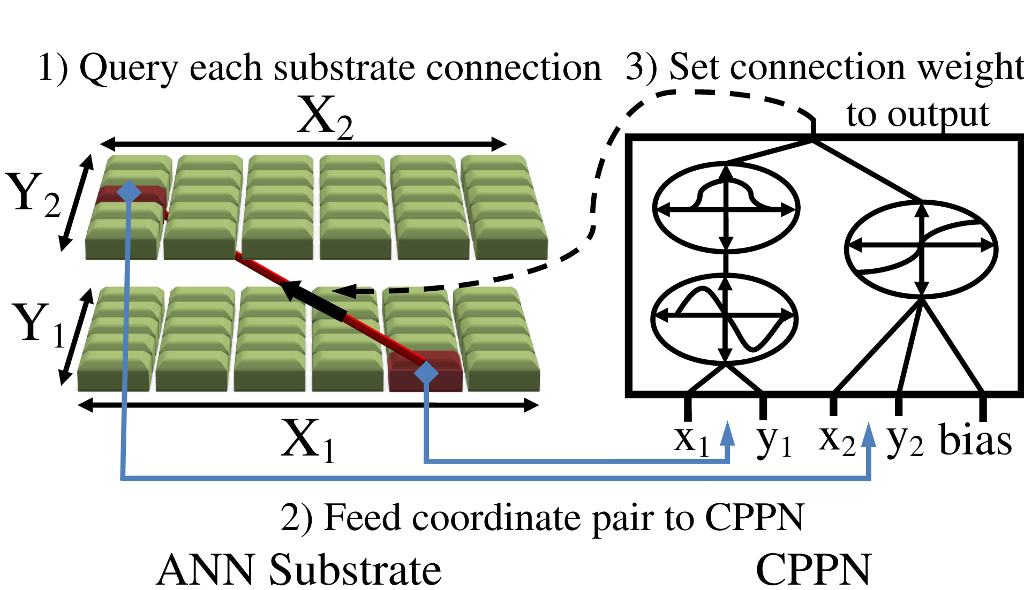
\includegraphics[width=\columnwidth]{figures/cppn}
\end{center}
\caption{HyperNEAT evolves the weights and topology of a CPPN (right). This CPPN is subsequently used to determine all of the weights between substrate nodes in a fully connected ANN (left). Finally, the ANN is used to compute the solution to the desired problem. This three stage process form the core of HyperNEAT. CPPNs are said to be geometrically aware because when they compute the weights of the associated ANN, they are given the geometric location of both the input and output node in the ANN.}
\label{fig:cppn}
\end{figure}

Having covered the basics of HyperNEAT, we now discuss the specifics of our approach including game screen processing and self identification.

\commentm{May need something here about how we attach a game screen to the input layer of the ANN.}

\section{Approach}
\label{sec:approach}
In this section we describe the details of our approach -- the main points are the manner in which the raw Atari game screen is processed to form an overhead representation amenable to HyperNEAT and the Condor framework used to parallelize the evaluation of individuals.

\subsection{Visual Processing}
\commentp{I am not sure how much visual processing naddaf did. If it was similar then we need to cite him}For nearly any machine learning problem, the question of how to encode the state space is of great importance. Following Verbancsics' example, we use an overhead object representation of the current game screen. Since we are given only the raw pixels of the screen as input, we design a simple visual processing stack which identifies objects and game entities without a priori knowledge of a specific game. A graphical depiction of this stack is shown in Figure \ref{fig:visproc}.

\begin{figure*}[htp]
\begin{center}
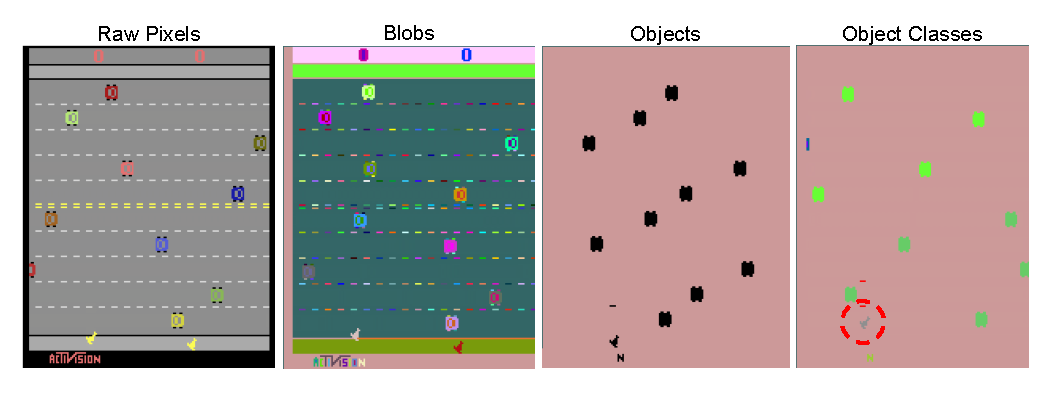
\includegraphics[width=\textwidth]{figures/AtariArch}
\end{center}
\caption{Visual Processing Architecture applied to the game Freeway. Raw pixels the game screen are displayed on the left. Next, contiguous pixels of the same color are merged into blobs. Objects are then extracted by merging adjacent blobs which exhibit constant velocity over the last two frames. Next, objects are clustered into object classes based on a pixel similarity score. Two main object classes are found -- cars facing left and cars facing right. Finally, self detection successfully identifies the chicken blob as the agent and colors it gray (circled in a red dashed line in rightmost screen).}
\label{fig:visproc}
\end{figure*}

Visual processing begins at the raw pixels of the game screen. We perform image segmentation in which adjacent raw pixels with similar colors are combined to form blobs. Next, blob merging occurs which outputs a set of current objects on screen. The process of blob merging examines all of the recently discovered blobs and compares them with equivalent blobs in the last frame in order to compute a velocity for each blob. Blobs are matched between screen using pixel similarity and velocity is computed by measuring the displacement of blob centroids. Once each blob is assigned a velocity, adjacent blobs with the same non-zero velocity are merged into objects. \commentp{added a line here} Objects which are too small or become stationary are thrown out. These checks help to reduce the number of false positives in cases where irrelevant components in the game screen are detected as objects.

Finally, objects are clustered into object classes or prototypes. Specifically, the shape of each pair of objects is compared and if found to exceed a threshold (97\% pixel match in these experiments), the objects were said to belong to the same class. Pixel similarity between two objects is computed by comparing the presence of absence \commentp{wait, what?} of pixels relative to each object's bounding box. As the object classes image in Figure \ref{fig:visproc} indicates, different object classes were discovered for the cars at the bottom half of the screen, cars at the top half of the screen, chicken, and lane separators. 

\commentp{added a line here} To reduce the number of spurious prototypes, prototypes are only passed to the next stage of the approach only when 25 instances of that prototype have been seen without a gap of more than 3 frames. In the example in Figure \ref{fig:visproc}, this check helps removes prototypes for objects created when the cars are at the edge of the screen and interact with the chicken. If a prototype fails this check then it is removed. If a prototype passes this check, a unique number is incrementally assigned to each prototype starting at 1. 

It is assumed here that objects belong to the same class if their shape is relatively similar without taking color into consideration. This could be a false assumption in certain games where different objects may have similar shapes bud different colors. However we have yet to encounter such a game.

\subsection{Self Identification}
The self detection step is meant to identify the location of an on-screen entity which is being controlled. In the vast majority of Atari games, the player's actions affect the movement of some on-screen entity here termed the \textit{self}. Knowledge of the location of the \textit{self} is crucial to selecting an action, as described in Subsection \ref{sec:interface}. We use an approach based on information gain to identify a blob most likely to correspond to the \textit{self}. Pseudocode is given in Algorithm \ref{alg:idself}.

\begin{algorithm}
\caption{Identify Self}
\label{alg:idself}
\begin{algorithmic}[1]
  \STATE $possible\_actions \leftarrow $ set of actions applicable to this game
  \STATE $current\_blobs \leftarrow $ set of blobs in the current game frame
  \STATE $ActionHistory \leftarrow \{a_0...a_n\}$ %\COMMENT{Actions at time 0...n}
  \FOR{blob $b \in current\_blobs$}
  \STATE $vHist_b \leftarrow \{v_0...v_n\}$ %\COMMENT{Velocity of blob $b$ at each timestep in the history}
  %\STATE \COMMENT{Information entropy of $b$'s velocity history}
  \STATE $H_b \leftarrow H(vHistory)$ 
  \FOR{action $a \in possible\_actions$}
  %\STATE \COMMENT{set of $b$'s velocities for timesteps in which action $a$ was taken}
  \STATE $vHist_{(b|a)} \leftarrow [vHist_b[t] ~\forall_t: ActionHist[t] == a]$ 
  \STATE $H_{(b|a)} \leftarrow H(vHist_{(b|a)})$ %\COMMENT{Information entropy of $b$'s velocity history given action $a$ was taken}
  \ENDFOR
  \STATE $InfoGain_b \leftarrow H_b - sum_{a \in actions}(p_a * H_{(b|a)})$ %\COMMENT{$p_a$ is probability of action $a$ based on observed frequency} 
  \ENDFOR
  \RETURN $arg\_max_{b \in current\_blobs}(InfoGain_b)$ %\COMMENT{Return blob with max information gain}
\end{algorithmic}
\end{algorithm}

At a high level, we assume two things: first, there is a blob on screen which corresponds to the self. Second, we expect that this blob will move similarly whenever the same action is performed -- that is, whenever an action, say Joystick Up, is taken, we expect the resulting velocity of the self blob to have a similar value (e.g. blob.y\_velocity = -1). 

As input, in lines 1-3, the algorithm has access to the set of possible joystick and button actions applicable to the current game (this is typically a subset of the 18 possible actions present on the Atari console), a list of blobs detected in the current frame, and a history of the actions taken by the agent. Additionally, in line 5, we have accesss to the $(x,y)$ velocity history $vHist$ of every blob. Next, we compute the entropy of blob $b$'s velocity history. Entropy is calculated using the standard formulation: $H(X) = -\sum_{i=1}^n{p(x_i)*lg(p(x_i))}$. Taking entropy over a velocity history involves computing the probability that blob $b$'s velocity assumes a given $(x,y)$ velocity value. This is done using the empirically observed frequencies of each observed $(x,y)$ velocity value in $b$'s velocity history. A blob with highly random movement will exhibit a high information entropy over its full velocity history while a blob with highly regular movement will yield low entropy.

Having computed the information entropy over $b$'s full velocity history, we next examine each action individually and, in line 8, create $b$'s selective velocity history $vHist_{(b|a)}$. The selective velocity history simply filters the full velocity history by including only velocities which were observed in frames after which action $a$ was taken. For example, if $a = $ joystick left, then $vHist_{(b|a)}$ would only contain resultant velocities for frames in which $a$ was the action selected. In line 9, entropy is computed over $b$'s selective velocity history. This selective entropy $H_{(b|a)}$ should be low if it is the case that a given action reliably the blob to move in a certain direction.

\label{sec:interface}

\begin{figure*}
  \centering
  \subfloat[Object Classes]{\label{fig:classes}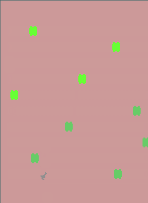
\includegraphics[width=0.196\textwidth]{figures/objClasses.png}}\hspace{.1in}
  \subfloat[Grid Overlay]{\label{fig:grid}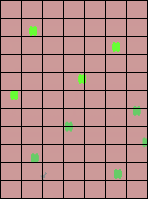
\includegraphics[width=0.2\textwidth]{figures/grid-overlay.png}}\hspace{.1in}
  \subfloat[ANN Input]{\label{fig:anninput}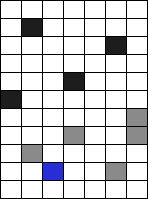
\includegraphics[width=0.2\textwidth]{figures/ann-input.png}}\hspace{.1in}
  \subfloat[ANN Output]{\label{fig:annoutput}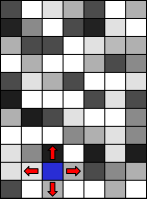
\includegraphics[width=0.2\textwidth]{figures/action-selection.png}}
 \caption{Interface between visual processing framework and the HyperNEAT ANN. Classes of objects are discretized into a grid whose cells are fed to the input nodes of the ANN via a map from object class to real number. After running the ANN, activations of the output layer in cells agent to the detected self are used to select which action the agent should take.}
 \label{fig:interface}
\end{figure*}

Finally, information gain is computed in line 11 by subtracting a frequency weighted sum of a blob's selective velocity entropies from the blob's full velocity entropy. If each of the selective entropies is low, as we expect for the self blob, this results in a high information gain. In line 13, the algorithm concludes by returning the blob with maximum information gain.

While this algorithm is generally successful in identifying the self blob, sometimes game dynamics break the assumption that actions result in similar velocities. For example, in the Freeway game, after colliding with a car, control is taken from the player and the chicken (\textit{self}) inadvertently moves down for several frames regardless of which actions the agent is executing. This results in irregular selective velocity histories and temporarily poorer identification of the self. However, in some sense the algorithm is correct in loosing confidence in an object over which it no longer has control.

\subsection{Atari-HyperNEAT Interface}

After extracting objects classes as well as the location of the self from the raw game screen, this information needs to be sent to HyperNEAT. As discussed in Section \ref{sec:hyperneat}, HyperNEAT evolves a CPPN which encodes an ANN. In this section we assume we have a fully connected 2-layer ANN whose weights have been specified by the CPPN. At a high level, information from the game screen needs to be translated to activations of nodes in the input layer of the ANN, and, after the network has been run in the standard feed-forward fashion, the activation of nodes on the output layer must be interpreted in order to select an action.

Figure \ref{fig:interface} shows an example of how objects classes are given as input to the substrate layer of the ANN. Since the ANN input nodes can only take real valued activations, each class of objects must be mapped to a real number. Thus we maintain a mapping from object classes to real values. Upon discovery of new object classes, real values are incrementally added to our map in a non-decreasing fashion. Next, since the ANN contains a 16x21 grid of input nodes, the raw game screen must also be discretized. Figure \ref{fig:grid} shows an example discretization of the game screen. Following this, each cell which contains an object is fed as input to the ANN with a real value corresponding to that object class's real value. Cells devoid of objects are given input activations of zero. The ANN is run in a standard feed-forward manner which produces activations of the nodes in the 16x21 output layer (Figure \ref{fig:annoutput}). In order to choose which action to take, we first locate cell corresponding to the location of the detected self object (colored blue in Figure \ref{fig:annoutput}). Having located this cell, we next examine its activation as well as the activations of the four adjacent cells (shown with red arrows) and select an action corresponding to the arrow in the highest of these five cells, or no-op action if the self square has the highest value. Future work involves extending this framework to support more complex actions such a button presses and combinations of joystick and button press actions.

Having described the interface between our visual processing framework and the HyperNEAT agent, we focus next on parallelizing the evaluation of individuals.

\subsection{Parallel Implementation}
\label{sec:condor}
The visual processing and self identification components of our code require some amount of processing time each frame. Depending on the game being played, evaluating a single individual can take anywhere between a few seconds to 5 minutes. Based on some initial experimental work, we estimated that we would need to run HyperNEAT for \textit{at least} 250 generations with 100 individuals per generation to obtain representative results. These parameters make it infeasible to run the entire computation on a single machine in a reasonable amount of time. To speed up evolution, we exploit the embarrassingly parallel nature of this approach by evaluating each individual on a separate machine. We make use of the Condor distributed processing cluster \cite{thain2005distributed} to run a massive number of Atari simulations in parallel. A similar framework has been used in the past to speed up the optimization of robot soccer agents in simulation using CMA-ES\cite{Urieli+MKBS:2010}. We have modified the original HyperNEAT implementation of \cite{verbancsics10} to run on the Condor cluster.

% To this end, we exploit the embarassingly parallel nature of the evaluating a number of individuals in a single generation. We use the Depending on the game being played in the Atari simulator, a single evaluation of an individual can last from anything between a few seconds to 2 or 3 minutes. While keeping the evolution parameters to as low as 100 individuals and 300 generations, it is still not possible to obtain results in sufficient time on a single machine. To mitigate this problem, we exploit the embarassingly parallel nature of evaluating individuals. We have modifed the HyperNEAT codebase to run on the Condor cluster, by adapting the framework developed by Yinon Bentor and Patrick MacAlpine.\footnote{This framework was initially developed in a previous iteration of the CS394N class. Since then it has been used by the AustinVilla Robot Soccer team for optimizing policy parameters for various soccer related tasks using evolutionary strategies such as CMA-ES.}

% \begin{figure*}[ht]
% \begin{center}
% 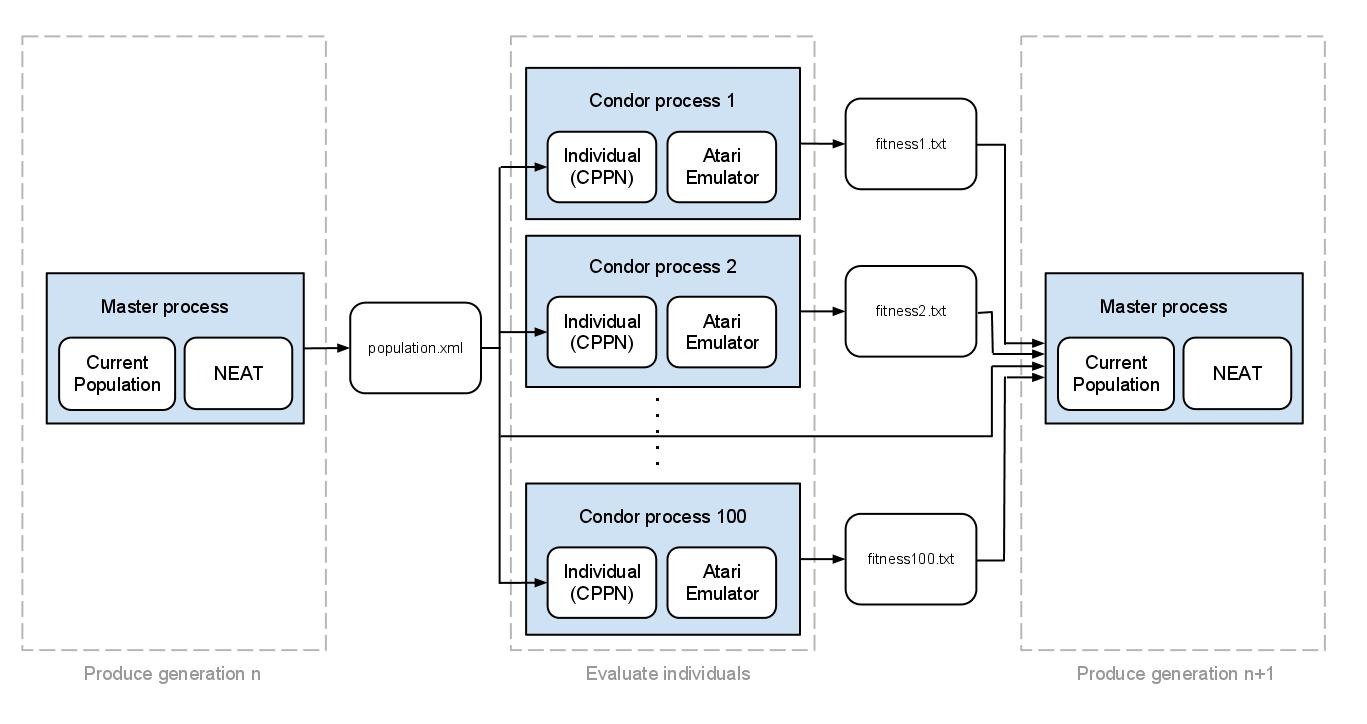
\includegraphics[width=\textwidth]{figures/CondorHyperNEAT}
% \end{center}
% \caption{Procedure for using HyperNEAT on the condor framework. An initial Master process is responsible for running NEAT and prodcuding successive generations. Condor jobs are initialized with each job being provided the population file and the id of th individual it is responsible for evaluating. Each job starts an instance of the Atari emulator and proceeds to evaluate the individual by playing the game using the policy defined by that individual. A fitness value is calculated, corresponding to the score obtained in the game and written out to file. This is read back by the Master process which then proceeds to use the fitness values to produce the next generation.}
% \label{fig:condor}
% \end{figure*}

\begin{figure}[ht]
\begin{center}
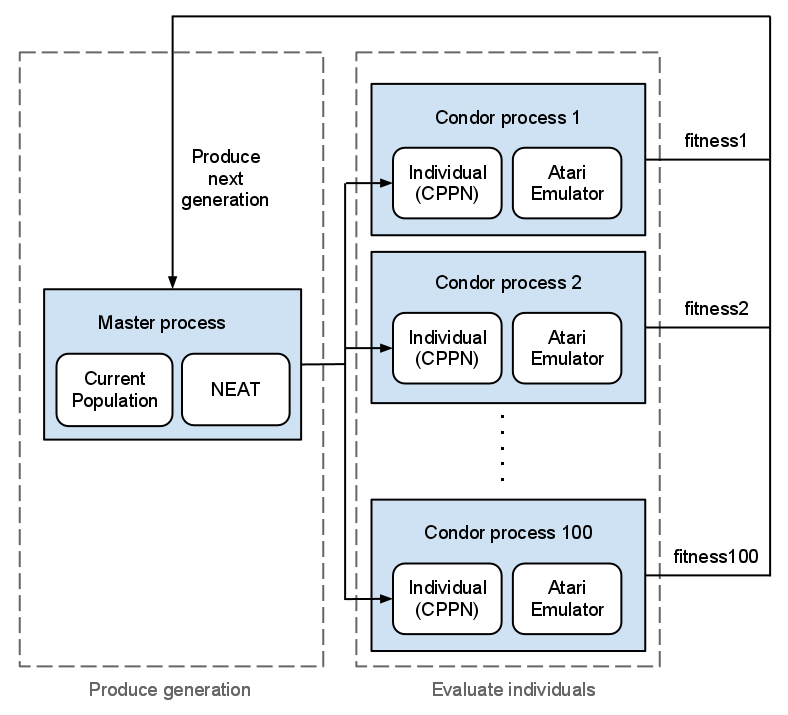
\includegraphics[width=\columnwidth]{figures/condor-hyperneat-small.png}
\end{center}
\caption{Parallel evaluations on the Condor framework}
\label{fig:condor}
\end{figure}

Figure \ref{fig:condor} details how parallel evaluations are performed using the Condor cluster. Once a generation is produced, all the individuals of that generation are evaluated on separate machines in parallel. After all evaluations have been completed, the fitness values are gathered and a new generation is produced. This process is then repeated for each successive generation. 

We detected a practical problem while using the framework; certain fitness evaluations do not complete and are assigned the minimum score. As a result, some individuals may be lost before maturing enough to improve other members of the population. Although such a situation is not ideal, we believe the evolutionary process to be robust enough to counter it. This hypothesis is corroborated by the steady increase of the average champion fitness in our experiments (see Fig. \ref{fig:asterix-curve}). 

\section{Results}
\label{sec:results}
In this section, we provide results obtained from applying HyperNEAT on two Atari games, \textit{Freeway} and \textit{Asterix}. The experimental setup was same for both Freeway and Asterix: HyperNEAT was run for 250 generations, with 100 individuals each generation and a substrate resolution of 16x21. All individuals were evaluated on the Atari simulator using the same random seed. We have averaged results across multiple runs of the HyperNEAT evolution and compare them with previous results obtained using reinforcement learning \cite{naddaf10}. We present the fitness values of the best individual averaged across all the runs, as well as the overall best individual found. In Table 1, BASS, DISCO, and RAM are gradient descent Sarsa$(\lambda)$ agents with linear function approximation. These methods use state representations corresponding to the sub-sampled screen image, objects on screen, and console ram respectively. We also compare against results obtained from an agent taking random actions each step \cite{naddaf10}. 

\subsection {Freeway}

Freeway is an Atari game similar to the arcade game \textit{Frogger}. The player controls a chicken with the objective of reaching the top of the highway while avoiding cars (see Fig. \ref{fig:visproc}). The player receives a score of 1 if the chicken reaches the top of the highway, and the chicken moves back to the bottom of the screen. If the chicken gets hit by a car, it gets pushed down by a fixed small distance. The game ends after two minutes of game-play. There are three possible actions that the player may use in Freeway: \textit{Up}, \textit{Down}, and \textit{No-Action}.

\begin{figure}[ht]
\begin{center}
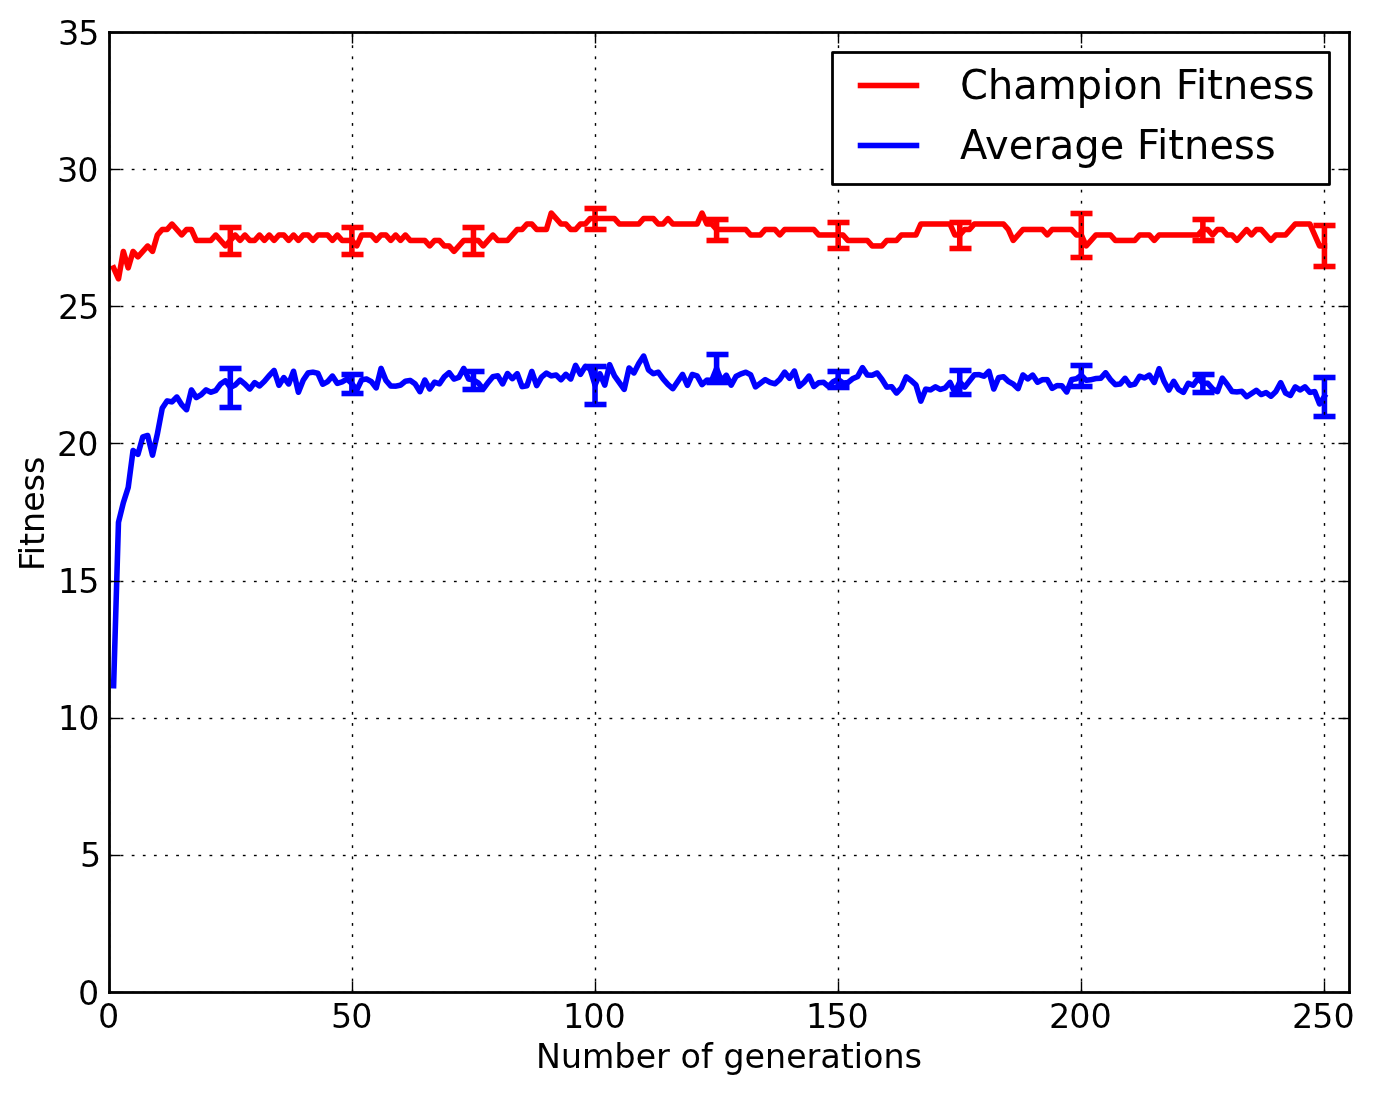
\includegraphics[width=\columnwidth]{figures/freeway-results.png}
\end{center}
\caption{The average fitness of the population along with the champion fitness at each generation in Freeway. Error bars represent standard deviation.}
\label{fig:freeway-curve}
\end{figure}

% \ref{tab:results-table} points incorrectly to 6?
Average fitness of the population and the champion fitness along the learning process can be seen in Fig. \ref{fig:freeway-curve}. Results were averaged across 5 runs of HyperNEAT evolution. Table 1 contrasts our approach with previous results. The most striking observation from these results is that reinforcement learning is unable to find a solution to the problem, whereas even the first generation in HyperNEAT produces a champion with a very high fitness (starting average champion fitness = 26.4). We believe that reinforcement learning has to perform a large number of exploratory actions before it can reach the goal state at the top, and succumbs to the highly delayed nature of the reward in this game. On the other hand, all individuals in HyperNEAT are produced by randomly initialized CPPNs. Due to the nature of CPPNs, at least a few individuals have the propensity to always take the \textit{Up} action and obtain a large fitness at the outset. Evolution helps individuals to learn fairly quickly to avoid cars over the next 50 generations, which can be seen by the slight increase in champion and average fitness.

\subsection {Asterix}
In Asterix, the player controls a unit called Asterix with the objective of collecting magic potions and avoiding \textit{lyres}. Both the magic potions and the lyres move across the screen around Asterix. Each time Asterix collects a magic potion, the player receives a score of 50. The game is over when the Asterix touches a lyre. Asterix can take five possible actions: \textit{Up}, \textit{Down}, \textit{Left}, \textit{Right}, and \textit{No-Action}.''

\begin{figure}[ht]
\begin{center}
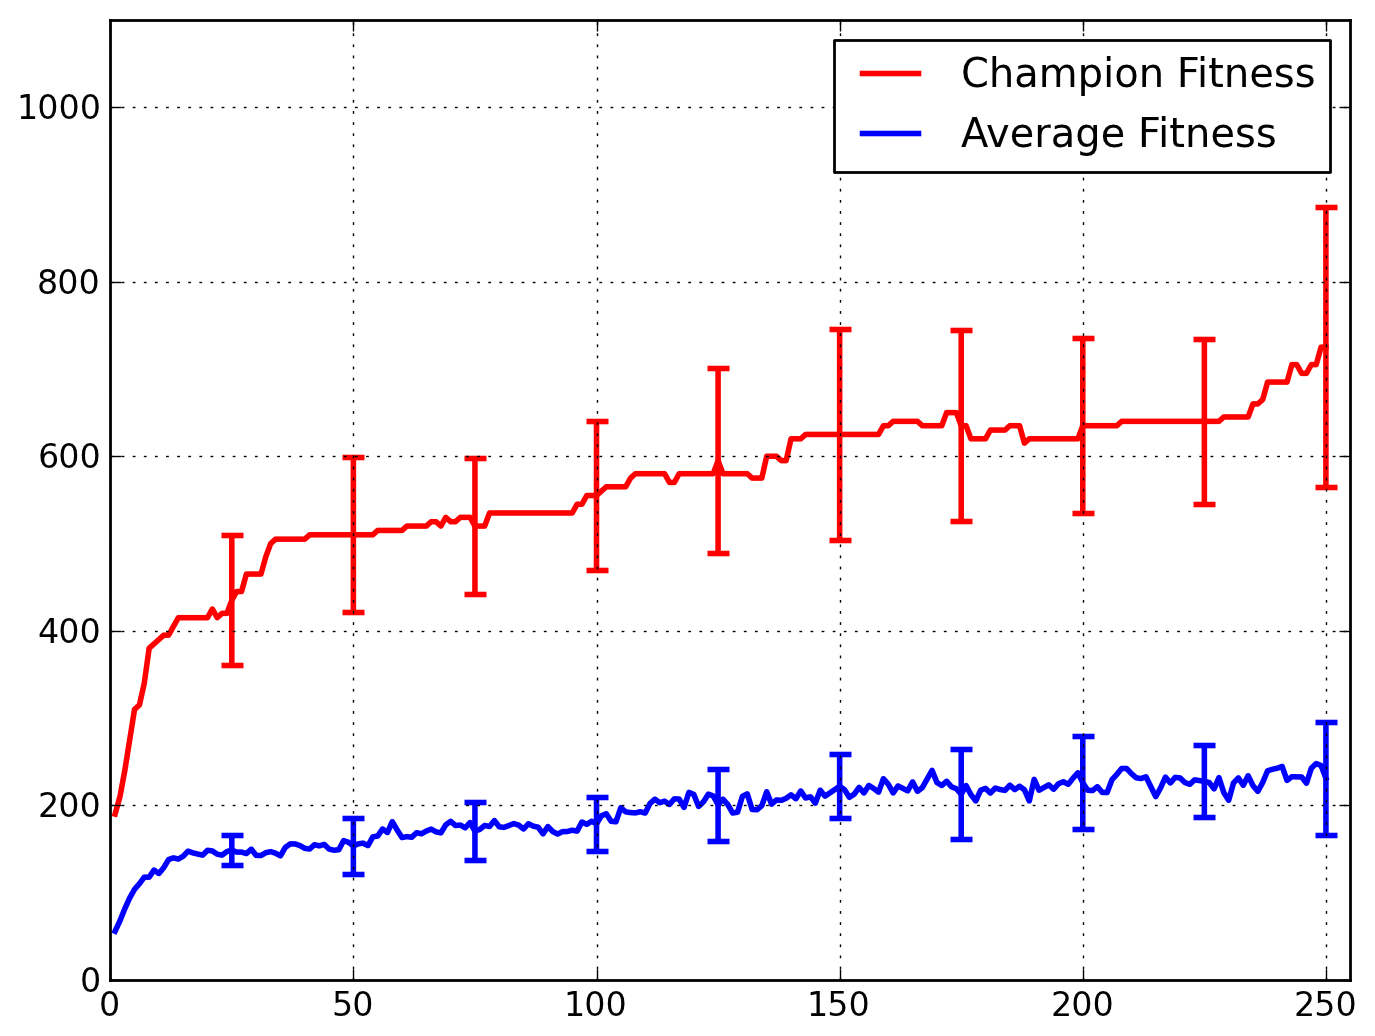
\includegraphics[width=\columnwidth]{figures/asterix-results.png}
\end{center}
\caption{The average fitness of the population along with the champion at each generation in the Asterix game. Error bars represent standard deviation}
\label{fig:asterix-curve}
\end{figure}

Average fitness of the population and the champion fitness along the learning process can be seen in Fig. \ref{fig:asterix-curve}. Results for Asterix were averaged across 10 runs of HyperNEAT evolution. Table 1 contrasts our approach with previous results. The results for Asterix are qualitatively different from Freeway in a number of ways:
\begin{itemize}
\item
Random exploration obtains non-zero reward in Asterix as Asterix inadvertently collects magic potions during random motion. Reinforcement Learning approaches can bootstrap from this information and learn to become statistically better than random.
\item
Champions from HyperNEAT evolution start at close to random performance (starting average champion fitness = 190) and improve their performance to the same level as that of reinforcement learning approaches within 50 generations. 
\item
The learning process steadily improves the fitness through the entirety of 250 generations. This demonstrates the power of using CPPNs at representing good policies for this game. Secondly, it also shows the ability of HyperNEAT to learn better CPPNs.
\end{itemize}

%Results from the Asterix game are summarized in Figure \ref{fig:asterix-curve} and Table 1. Unlike the Freeway game, the champion fitness curve shows significant improvement accross successive generations. Secondly, the champion fitness reaches a high of 750 before dropping down to around the 550 mark. We suspect that our Condor implementaion is responsible, and that the champion was lost to an incomplete Condor job (see Section \ref{sec:condor}). We hope to rectify this issue in the future by making our framework more robust. In contrast to the Freeway game, RL methods perform decently well in this domain. Initial exploration probably causes the agent to learn to stay away from the sprites much faster in this case. However HyperNEAT still outperforms RL based methods. On the other hand, HyperNEAT does not perform as well as a human player. We attribute this to the higher complexity of the game, as well as multiple object classes (which is something we are still working on). 

\begin{table}
\begin{center}
\begin{tabular}{|l|c|c|}
\hline
~ & \textbf{Freeway} & \textbf{Asterix} \\ \hline
\textbf{BASS} & 0 & 402 \\ \hline
\textbf{DISCO} & 0 & 301 \\ \hline
\textbf{RAM} & 0 & 545 \\ \hline
\textbf{Random} & 0 & 156 \\ \hline
\textbf{HyperNEAT(Average)} & 28.4 & 725 \\ \hline
\textbf{HyperNEAT(Best)} & 29 & 1000 \\ 
\hline
\end{tabular}
\end{center}
\label{tab:results-table}
\caption{Game scores obtained in the Freeway and Asterix games.}
\end{table}

\section{Future Work}
\label{sec:futurework}
While HyperNEAT learning proved successful on the Freeway and Asterix domains, many challenges remain for future work. First and foremost, we hope to make the framework applicable to a larger set of games. There are two main challenges in this regard -- first handling games with large numbers of possible actions and second handling games with many different object classes.

In Freeway and Asterix, like in Robocup Keepaway, there are relatively few classes of objects which matter: cars and the chicken for Freeway, potions and harps for Asterix, and takers and keepers for keepaway. Having a limited number of object classes permits an easy mapping from objects to substrate values -- for example, in Keepaway, keepers can be assigned values of 1 and takers values of -1. Having such few values allows HyperNEAT to easily differentiate different classes of objects and exhibit appropriate behaviors with respect to each object class, behaviors such as avoiding harps and collecting potions.

Discernment between object classes becomes less clear as the number of classes increases. In the worst case, if two opposite classes of objects (e.g. keepers and takers) get mapped to the same real value, HyperNEAT will be unable to distinguish between them and formulate appropriate strategies.

One possible solution to this problem is to create multiple layers of input substrate, with one layer for each class of objects. Figure \ref{fig:possiblearch} depicts this concept. Each new object class is given its own substrate layer which it exclusively populates. At runtime, each of the substrate layers is connected to the processing layer and run in a feed-forward manner. Additionally one more input would need to be added to the CPPN to specify which substrate was currently active. In this way, HyperNEAT would, with some additional computation costs, be able to encode an entirely different policy for an arbitrary number of object classes. 

The second area of future work involves engineering a better way to handle a large number of actions. In games like Freeway in which there are only a few actions (up, down, no-op), we can choose which action to take by examining values of the output nodes adjacent to the self node (as described in Section \ref{sec:interface}). This becomes more complicated when other actions such as button pressing are included. (Which node's value should be examined to decide if the button press action should be taken?) To address this issue, we hope to add another output layer above the processing layer. This additional output layer would have a single node for each of the possible actions in the game. Choosing which action to execute would then be as simple as finding action node with the highest value, and adding possible actions would reduce to adding extra nodes to this new layer. The top of Figure \ref{fig:possiblearch} shows a graphical depiction of this alternative architecture.

\begin{figure}[htp]
\begin{center}
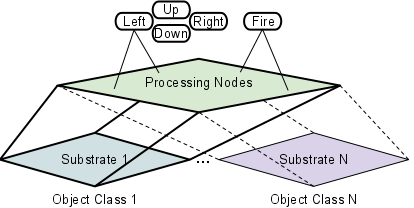
\includegraphics[width=\columnwidth]{figures/multiple-substrate.png}
\end{center}
\caption{Alternative architecture for handling variable numbers of object classes and actions. New object classes are assigned individual substrate layers. Additionally, above the processing level exists a node for each possible action. At runtime activations are propagated up from all $N$ substrate layers to the processing and action layers. Action selection involves picking which action node has the highest activation.}
\label{fig:possiblearch}
\end{figure}

\section{Conclusions}
\label{sec:conclusion}
In this work we have applied HyperNEAT to the novel domain of Atari games. Atari games exhibit geometric regularities in the two-dimensional space of the game screen which allows HyperNEAT to quickly learn effective policies. Rather than learning on raw pixels of the game screen, we first apply visual processing techniques to identify objects on screen. Next, these objects are provided as input to the HyperNEAT CPPN. Due to the computational overhead of visually processing each game screen, we utilize a parallel architecture to simultaneously evaluate multiple individuals. Results are presented for two Atari games, \textit{Freeway} and \textit{Asterix}. In both cases, HyperNEAT is shown to outperform previous benchmarks\cite{naddaf10} and in one case exceeds human level play. We expect that with relatively minor modifications, the framework presented here will be able to play arbitrary Atari games with zero manual reconfiguration. In closing, we hypothesize that none of the Atari games, in isolation, poses too great a learning challenge. However, it is our hope that a learning algorithm capable of playing a large number of these games without prior knowledge or reconfiguration would represent a non-trivial step towards an AI general and robust enough to begin to tackle the great diversity of tasks humans deal with on a daily basis.

%\end{document}  % This is where a 'short' article might terminate

%ACKNOWLEDGMENTS are optional
%% \section{Acknowledgments}
%% This section is optional; it is a location for you
%% to acknowledge grants, funding, editing assistance and
%% what have you.  In the present case, for example, the
%% authors would like to thank Gerald Murray of ACM for
%% his help in codifying this \textit{Author's Guide}
%% and the \textbf{.cls} and \textbf{.tex} files that it describes.

%
% The following two commands are all you need in the
% initial runs of your .tex file to
% produce the bibliography for the citations in your paper.
\bibliographystyle{abbrv}
\bibliography{hyperneat}  % sigproc.bib is the name of the Bibliography in this case
% You must have a proper ".bib" file
%  and remember to run:
% latex bibtex latex latex
% to resolve all references

\end{document}
